\documentclass[8pt]{beamer}

\usepackage{mathtools}

% For drawing automata
\usepackage{tikz}
\usetikzlibrary{automata, positioning, arrows.meta, shapes.multipart}

\tikzset{
    every state/.style={
        draw=black,
        thick,
        minimum size=1.2cm,
        inner sep=3pt,
        font=\small
    }
}
\usepackage{adjustbox}

\usetheme{Antibes}
\setbeamertemplate{footline}[frame number]

\begin{document}

\begin{frame}{Outine}
    \tableofcontents
\end{frame}

\AtBeginSection[ ]
{
    \begin{frame}{Outline}
        \tableofcontents[currentsection]
    \end{frame}
}

\section{ILP Ideas}
\begin{frame}{Notation}
    \begin{itemize}
        \item Let $M := \{1,\dotsc,N_m\}$ a lineraly ordered set of models
        \item Let $S := \{1,\dotsc,N_s\}$ a set of switches
        \item Let $\mathcal{P} := (P_i)_{i \in \{1,\dotsc,N_p\}}$ a family of paths
        \item For a path $P_i \in \mathcal{P}$ :
            \begin{itemize}
                \item We represent $P_i$ by its sequence of vertices (i.e. switches)
                \item Let $l_i$ the number of switches in $P_i$
                \item Let $s_i^k$ the k-th switch of the sequence $P_i$
            \end{itemize}
    \end{itemize}
\end{frame}

\begin{frame}{Ideas}
    \begin{table}
        \begin{tabular}{|c||c|c|}
            \hline
            ILP & Dependency & Nb. models per switch \\
            \hline \hline
            1 & Restrictive & $\leq 1$ \\
            \hline
            2 & Permisive & $\leq N$ \\
            \hline
            3 & Permisive & N/A \\
            \hline
        \end{tabular}
    \end{table}
\end{frame}

\begin{frame}{ILP 1}
    Variables : $X_{s \gets m}$ deploy model $m$ on switch $s$
    \begin{equation*}
        \begin{aligned}
            \mathrm{Min.} \quad & \sum_{s \in S} \sum_{m \in M} X_{s \gets m} \\[1em]
            \mathrm{S.t.}
            % Integrity
            \quad & \sum_{s \in P} X_{s \gets m} \geq 1
            \quad & \forall m \in M, \forall P \in \mathcal{P} \\
            % Dependency
            \quad & \sum_{k=1}^{j-1} X_{s_i^k \gets m} \geq X_{s_i^j\gets m'}
            \quad & \forall m < m',\forall i \in [N_p], \forall j \in [l_i]
        \end{aligned}
    \end{equation*}
\end{frame}

\begin{frame}{ILP 2}
    Variables : $X_{s \gets m}$ deploy model $m$ on switch $s$
    \begin{equation*}
        \begin{aligned}
            \mathrm{Min.} \quad & \sum_{s \in S} \sum_{m \in M} X_{s \gets m} \\[1em]
            \mathrm{S.t.}
            % Integrity
            \quad & \sum_{s \in P} X_{s \gets m} \geq 1
            \quad & \forall m \in M, \forall P \in \mathcal{P} \\
            % Dependency
            \quad & \sum_{k=1}^{j} X_{s_i^k \gets m} \geq X_{s_i^j \gets m'}
            \quad & \forall m < m',\forall i \in [N_p], \forall j \in [l_i]
        \end{aligned}
    \end{equation*}
\end{frame}

\begin{frame}{ILP 3}
    Let $\mathcal{M}$ the set of all subsets of $M$\\
    Let $M'_m := \{M' \in \mathcal{M} | m \in M'\}$\\
    Variables : $X_{s \gets M'}$ deploy all models $m \in M'$ with $M' \in \mathcal{M}$ on switch $s$
    \begin{equation*}
        \begin{aligned}
            \mathrm{Min.} \quad & \sum_{s \in S} \sum_{M' \in \mathcal{M}} |M'|X_{s \gets M'} \\[1em]
            \mathrm{S.t.}
            % Integrity
            \quad & \sum_{s \in P} \sum_{M' \in M'_m} X_{s \gets M'} \geq 1
            \quad & \forall m \in M, \forall P \in \mathcal{P} \\
            % Dependency
            \quad & \sum_{k=1}^{j-1} \sum_{A \in M'_m} X_{s_i^k \gets A} \geq \sum_{B \in M'_{m'}} X_{s_i^j\gets B}
            \quad & \forall m < m',\forall i \in [N_p], \forall j \in [l_i]
        \end{aligned}
    \end{equation*}
\end{frame}


\section{Logic, states, and other stuff}
\begin{frame}{Discussions, reflexions, assumptions, and deductions}{Part 1}
    \begin{exampleblock}{Assumptions}
        Given $n$ models.
        From the model sequencing we can assume:
        \begin{itemize}
            \item Models are linearly ordered from best to worst
                (i.e. \(m_1<\dotsb<m_n\))
        \end{itemize}
        By best to worst we mean, given \(m_i<m_j\), we will consider a result
        from \(m_i\) as more valueable than a result of the same type from \(m_j\).
    \end{exampleblock}

    \begin{block}{Notation}
        A model \(m_i\) can produce a result:
        \begin{itemize}
            \item PL-U \(\implies\) The packet level class is not in \(m_i\)
            \item PL-K \(\implies\) The packet level class is in \(m_i\)
            \item FL-U \(\implies\) The flow level class is not in \(m_i\)
            \item FL-K \(\implies\) The flow level class is in \(m_i\)
        \end{itemize}
    \end{block}
\end{frame}

\begin{frame}{Discussions, reflexions, assumptions, and deductions}{Part 2}
    \begin{exampleblock}{Assumptions for both assertions}
        \begin{itemize}
            \item A flow of packets goes through models following the order
                provided by sequencing.
            \item If the local result is FL-K, we initiate the process to
                populate tables accordingly and clear registers of the switches
                on the path of the flow.
        \end{itemize}
    \end{exampleblock}

    \begin{alertblock}{Assertion A}
        A result of type PL can only be produced locally if it was previously classified as PL-Unknown or FL-Unknown
    \end{alertblock}

    \begin{alertblock}{Assertion B}
        A result of type FL can only be produced locally if it was previously classified as FL-Unknown
    \end{alertblock}
\end{frame}

\begin{frame}{Discussions, reflexions, assumptions, and deductions}{Part 3}
    \begin{proof}[Proof of assertion A (by contraposition)]
        Assuming previous classification is not PL-U and not FL-U.
        I show that a result of type PL cannot be produced locally.
        We have 2 cases :
        \begin{enumerate}
            \item Previous result is FL-K : Trivial
            \item Previous result is PL-K : \\
                A local result PL-K' would overwitre PL-K. This contradicts
                our assumation that we value more a result from an earlier model.
        \end{enumerate}
    \end{proof}
\end{frame}

\begin{frame}{Discussions, reflexions, assumptions, and deductions}{Part 4}
    \begin{proof}[Proof of assertion B]
        Assuming previous classification is not FL-Unknown.
        I show that a result of type FL cannot be produced locally.
        We have 3 cases :
        \begin{enumerate}
            \item Previous result is FL-K : Trivial
            \item Previous result is PL-K : \\
                For a contradiction, assume a result of type FL we can be produced locally
                and that we use this result.
                But some point, the previous result must become a FL but it
                is overwritten by the local result. This contradicts our
                assumption that we value more results produced by previous models.
            \item Previous result is PL-U : Same reasoning as previous item.
        \end{enumerate}
    \end{proof}
\end{frame}

\begin{frame}{Tracking the state of flow's pkt classification type inside a switch}
    \begin{adjustbox}{width=\textwidth}{
        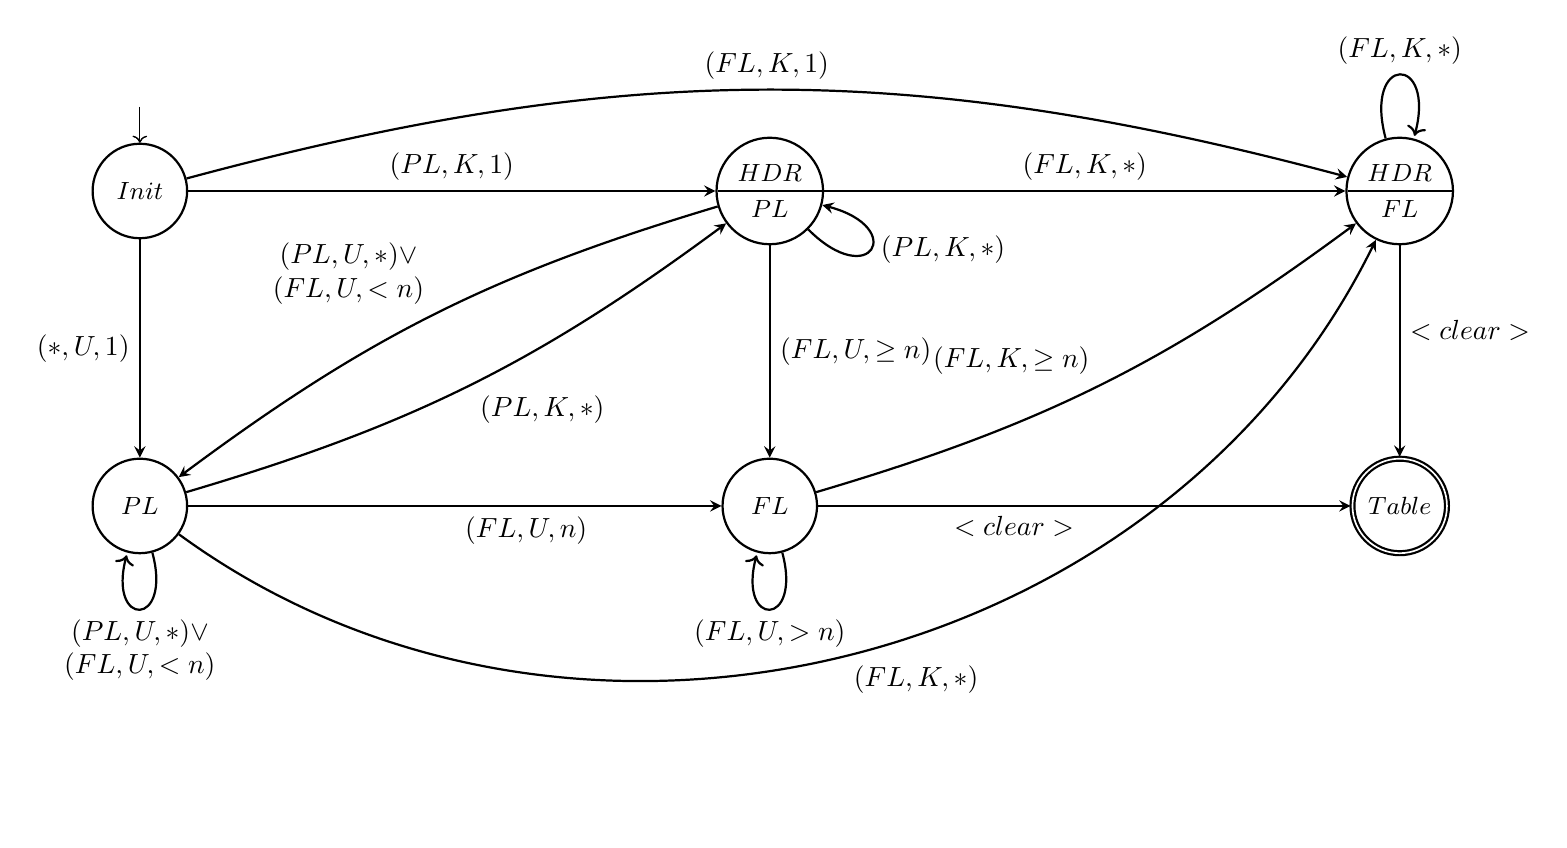
\begin{tikzpicture}
            % Help lines :
            % \draw [help lines] (-1,1) grid (17,-9);

            % States
            \node (init) [
                state,
                initial,
                initial above,
                initial text={},
            ] at (0,0) {$Init$};
            \node (hdrPL) [
                state with output,
            ] at (8,0) {$HDR$ \nodepart{lower} $PL$};
            \node (hdrFL) [
                state with output,
            ] at (16,0) {$HDR$ \nodepart{lower} $FL$};
            \node (pl) [
                state,
            ] at (0,-4) {$PL$};
            \node (fl) [
                state,
            ] at (8,-4) {$FL$};
            \node (table) [
                state,
                accepting,
            ] at (16,-4) {$Table$};

            % Edges
            \path [-stealth, thick]
                % Out of init
                (init) edge node [above] {$(PL,K, 1)$} (hdrPL)
                (init) edge [bend left=15] node [above] {$(FL,K,1)$} (hdrFL)
                (init) edge node [left,align=center] {$(*,U,1$)} (pl)

                % Out of hdrPL
                (hdrPL) edge[out=315, in=345, looseness=8] node[right] {$(PL,K,*)$} (hdrPL)
                (hdrPL) edge node [above] {$(FL,K,*)$} (hdrFL)
                (hdrPL) edge [bend right=10] node [above left,align=center] {$(PL,U,*)\lor$\\$(FL,U,<n)$} (pl)
                (hdrPL) edge node [right] {$(FL,U,\ge n)$} (fl)

                % Out of hdrFL
                (hdrFL) edge [loop above] node [above] {$(FL,K, *)$}()
                (hdrFL) edge node [above right] {$<clear>$} (table)

                % Out of PL
                (pl) edge [loop below] node [below,align=center] {$(PL,U,*)\lor$\\$(FL,U,<n)$}()
                (pl) edge [bend right=10] node [below right] {$(PL,K,*)$} (hdrPL)
                (pl) edge [bend right=50] node [below right] {$(FL,K,*)$} (hdrFL)
                (pl) edge node [below right] {$(FL,U,n)$} (fl)

                % Out of FL
                (fl) edge [loop below] node [below] {$(FL,U,>n)$}()
                (fl) edge [bend right=10] node [above left] {$(FL,K,\ge n)$} (hdrFL)
                (fl) edge node [below left] {$<clear>$} (table)
            ;
        \end{tikzpicture}
    }
    \end{adjustbox}
\end{frame}

\begin{frame}{Actions taken inside a switch when receiving a packet}{Part 1 : Entering state PL}
    \begin{adjustbox}{width=\textwidth}
        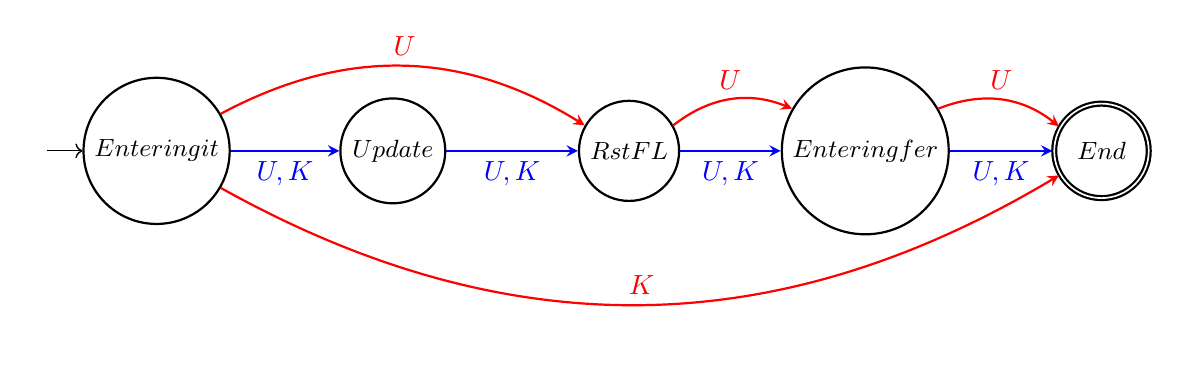
\begin{tikzpicture}[node distance = 3cm, on grid, auto]
            % Help lines :
            %\draw [help lines] (-1,1) grid (10,-9);

            % States
            \node (init) [
                state,
                initial,
                initial left,
                initial text={},
            ] {$Enteringit$};
            \node (update) [
                state,
                right = of init
            ] {$Update$};
            \node (rstFl) [
                state,
                right = of update,
            ] {$RstFL$};
            \node (infer) [
                state,
                right = of rstFl,
            ] {$Enteringfer$};
            \node (end) [
                state,
                accepting,
                right = of infer,
            ] {$End$};

            % Without collision
            \path [-stealth, thick, color=blue]
                (init) edge node [below] {$U,K$} (update)
                (update) edge node [below] {$U,K$} (rstFl)
                (rstFl) edge node [below] {$U,K$} (infer)
                (infer) edge node [below] {$U,K$} (end)
            ;

            % With collision
            \path [-stealth, thick, color=red]
                % PL-U
                (init) edge [bend left] node [above] {$U$} (rstFl)
                (rstFl) edge [bend left] node [above] {$U$} (infer)
                (infer) edge [bend left] node [above] {$U$} (end)

                % PL-K
                (init) edge [bend right] node [above] {$K$} (end)
            ;
        \end{tikzpicture}
    \end{adjustbox}
\end{frame}

\begin{frame}{Actions taken inside a switch when receiving a packet}{Part 2 : Entering state FL}
    \begin{adjustbox}{width=\textwidth}
        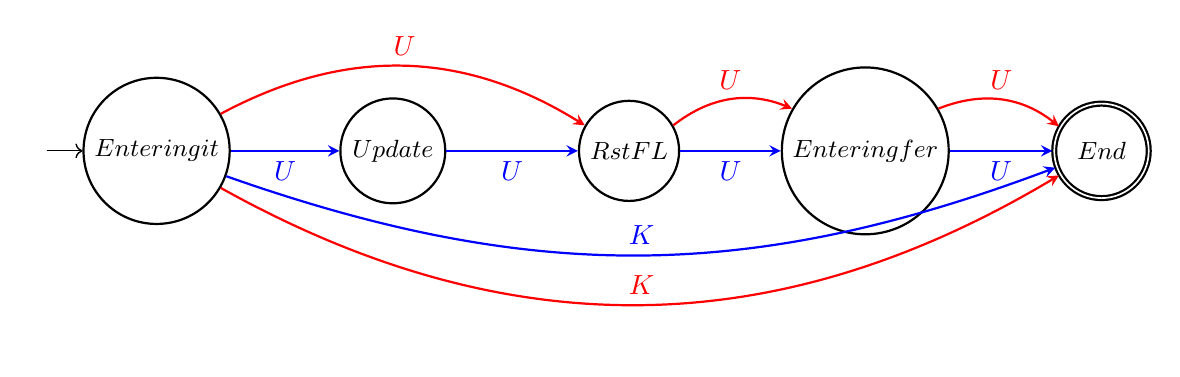
\begin{tikzpicture}[node distance = 3cm, on grid, auto]
            % Help lines :
            %\draw [help lines] (-1,1) grid (10,-9);

            % States
            \node (init) [
                state,
                initial,
                initial left,
                initial text={},
            ] {$Enteringit$};
            \node (update) [
                state,
                right = of init
            ] {$Update$};
            \node (rstFl) [
                state,
                right = of update,
            ] {$RstFL$};
            \node (infer) [
                state,
                right = of rstFl,
            ] {$Enteringfer$};
            \node (end) [
                state,
                accepting,
                right = of infer,
            ] {$End$};

            % Without collision
            \path [-stealth, thick, color=blue]
                % FL-U
                (init) edge node [below] {$U$} (update)
                (update) edge node [below] {$U$} (rstFl)
                (rstFl) edge node [below] {$U$} (infer)
                (infer) edge node [below] {$U$} (end)

                %FL-K
                (init) edge [bend right=20] node [above] {$K$} (end)
            ;

            % With collision
            \path [-stealth, thick, color=red]
                % FL-U
                (init) edge [bend left] node [above] {$U$} (rstFl)
                (rstFl) edge [bend left] node [above] {$U$} (infer)
                (infer) edge [bend left] node [above] {$U$} (end)

                % FL-K
                (init) edge [bend right] node [above] {$K$} (end)
            ;
        \end{tikzpicture}
    \end{adjustbox}
\end{frame}

\begin{frame}{Actions taken inside a switch when receiving a packet}{Part 3 : Entering state HDR\_PL}
    \begin{adjustbox}{width=\textwidth}
        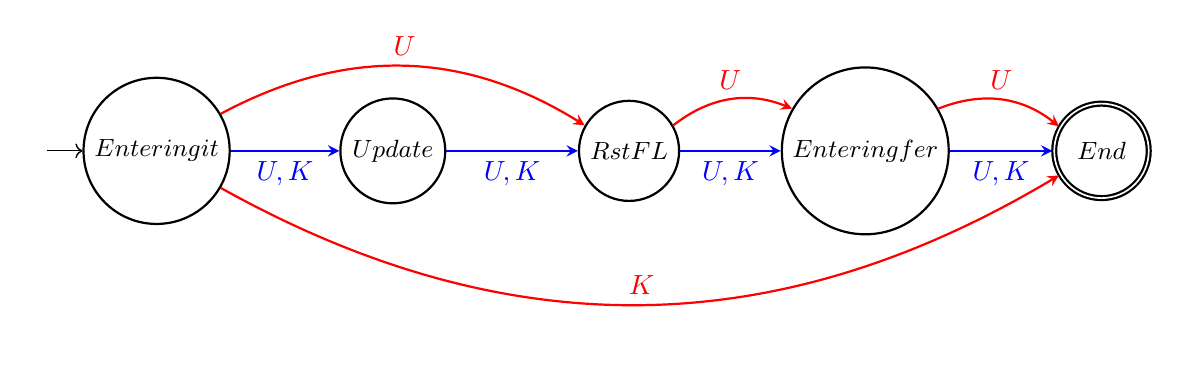
\begin{tikzpicture}[node distance = 3cm, on grid, auto]
            % Help lines :
            %\draw [help lines] (-1,1) grid (10,-9);

            % States
            \node (init) [
                state,
                initial,
                initial left,
                initial text={},
            ] {$Enteringit$};
            \node (update) [
                state,
                right = of init
            ] {$Update$};
            \node (rstFl) [
                state,
                right = of update,
            ] {$RstFL$};
            \node (infer) [
                state,
                right = of rstFl,
            ] {$Enteringfer$};
            \node (end) [
                state,
                accepting,
                right = of infer,
            ] {$End$};

            % Without collision
            \path [-stealth, thick, color=blue]
                (init) edge node [below] {$U,K$} (update)
                (update) edge node [below] {$U,K$} (rstFl)
                (rstFl) edge node [below] {$U,K$} (infer)
                (infer) edge node [below] {$U,K$} (end)
            ;

            % With collision
            \path [-stealth, thick, color=red]
                % PL-U
                (init) edge [bend left] node [above] {$U$} (rstFl)
                (rstFl) edge [bend left] node [above] {$U$} (infer)
                (infer) edge [bend left] node [above] {$U$} (end)

                % PL-K
                (init) edge [bend right] node [above] {$K$} (end)
            ;
        \end{tikzpicture}
    \end{adjustbox}
\end{frame}

\begin{frame}{Actions taken inside a switch when receiving a packet}{Part 4 : Entering state HDR\_FL}
    \begin{adjustbox}{width=\textwidth}
        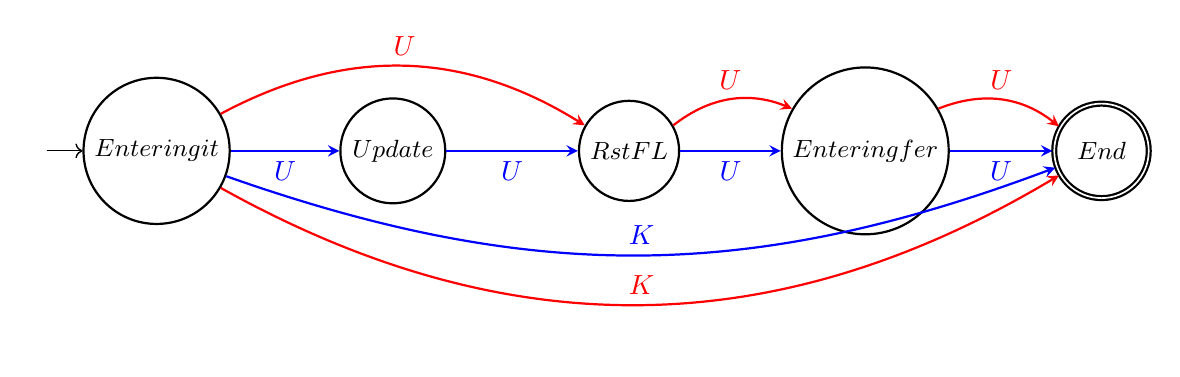
\begin{tikzpicture}[node distance = 3cm, on grid, auto]
            % Help lines :
            %\draw [help lines] (-1,1) grid (10,-9);

            % States
            \node (init) [
                state,
                initial,
                initial left,
                initial text={},
            ] {$Enteringit$};
            \node (update) [
                state,
                right = of init
            ] {$Update$};
            \node (rstFl) [
                state,
                right = of update,
            ] {$RstFL$};
            \node (infer) [
                state,
                right = of rstFl,
            ] {$Enteringfer$};
            \node (end) [
                state,
                accepting,
                right = of infer,
            ] {$End$};

            % Without collision
            \path [-stealth, thick, color=blue]
                % FL-U
                (init) edge node [below] {$U$} (update)
                (update) edge node [below] {$U$} (rstFl)
                (rstFl) edge node [below] {$U$} (infer)
                (infer) edge node [below] {$U$} (end)

                %FL-K
                (init) edge [bend right=20] node [above] {$K$} (end)
            ;

            % With collision
            \path [-stealth, thick, color=red]
                % FL-U
                (init) edge [bend left] node [above] {$U$} (rstFl)
                (rstFl) edge [bend left] node [above] {$U$} (infer)
                (infer) edge [bend left] node [above] {$U$} (end)

                % FL-K
                (init) edge [bend right] node [above] {$K$} (end)
            ;
        \end{tikzpicture}
    \end{adjustbox}
\end{frame}

\end{document}
